\documentclass[12pt]{article}
\usepackage{geometry}
\usepackage{tikz}
\geometry{margin=1in}

\usetikzlibrary{arrows.meta,calc}
\definecolor{accent}{RGB}{0,90,160}
\definecolor{softgray}{RGB}{230,230,230}

\tikzset{
    shaft/.style={thick},
    forcevec/.style={->,thick,accent},
    couplevec/.style={->,thick,accent},
    refpoint/.style={circle,fill=black,inner sep=1.5pt},
    labelpt/.style={circle,fill=black,inner sep=1.2pt},
    axisline/.style={thin},
    boundregion/.style={fill=softgray,draw=none,opacity=0.5}
}

\title{\Large\bfseries
What Inverse Dynamics Really Tells Us About the Hands:\\[4pt]
A Practical Guide for Coaches and Practitioners}

\author{2025}
\date{}

\begin{document}
\maketitle

\begin{abstract}
Inverse dynamics is a popular tool in golf research.  
It takes the motion of the club and, using physics, works backwards to estimate the overall force and torque that must have been applied to create that motion.  

Because the results are often shown as a single ``force and torque at the hands'', it is tempting to read them as literal measurements of how the golfer pushed, pulled, and twisted the club.  
This is not what inverse dynamics provides.

This article explains, in coach-friendly language and diagrams, what inverse dynamics can and cannot tell us about hand action.  
We focus on the two-handed grip, why the system is mechanically ambiguous, and how to use inverse-dynamics results responsibly when thinking about technique, coaching, or equipment.
\end{abstract}

\tableofcontents
\newpage

%==========================================================================
\section{What Inverse Dynamics Does in Simple Terms}
%==========================================================================

Imagine you know exactly how the club moved during the swing: where it was, how fast it was moving, and how quickly it was speeding up or slowing down.  
Inverse dynamics takes that motion and asks:

\begin{quote}
    \emph{``What overall push and twist would be needed to make the club move like this, if they were applied at a specific point on the club?"}
\end{quote}

The output is:
\begin{itemize}
    \item one overall \textbf{force}, and
    \item one overall \textbf{twisting action} (often called a \emph{couple} or \emph{torque})
\end{itemize}
at the chosen point, usually the midpoint between the hands.

This is a very useful summary of how the club was loaded, but it is not a direct snapshot of what each hand did.

%==========================================================================
\section{A Single Force Can Look Like a Twist}
%==========================================================================

A key idea is that a \emph{push applied away from the analysis point} will always look like a combination of:
\begin{itemize}
    \item a push at the analysis point, plus
    \item a twist around the analysis point.
\end{itemize}

\subsection*{Diagram 1: One off-center push becomes push + twist at the midpoint}

\begin{center}
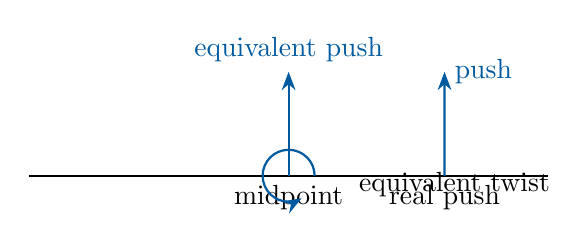
\begin{tikzpicture}[scale=1.1,>=Stealth]
    % Club
    \draw[shaft] (-3,0) -- (3,0);
    % Midpoint
    \fill[refpoint] (0,0) circle;
    \node[below] at (0,0) {midpoint};
    % Real force point
    \coordinate (fp) at (1.8,0);
    \fill[labelpt] (fp) circle;
    \node[below] at (fp) {real push};
    % Real force
    \draw[forcevec] (fp) -- (1.8,1.2) node[right] {push};
    % Equivalent at midpoint
    \draw[forcevec] (0,0) -- (0,1.2) node[above] {equivalent push};
    \draw[couplevec] (0.3,0) arc (0:300:0.3);
    \node[right] at (0.7,-0.1) {equivalent twist};
\end{tikzpicture}
\end{center}

So even if the golfer did \emph{not} try to twist the club, the reported ``torque'' at the midpoint may be nonzero simply because the push did not act exactly at that point.

\begin{quote}
\textbf{A twist in the inverse-dynamics output does not automatically mean the player twisted the club.}
\end{quote}

%==========================================================================
\section{Two Hands Make the System Ambiguous}
%==========================================================================

With one hand on the club, the situation is simpler.  
With two hands, we get a closed system: the left hand, the club, and the right hand all push and pull on each other in a loop.

\subsection*{Diagram 2: Two hands, many ways to create the same club motion}

\begin{center}
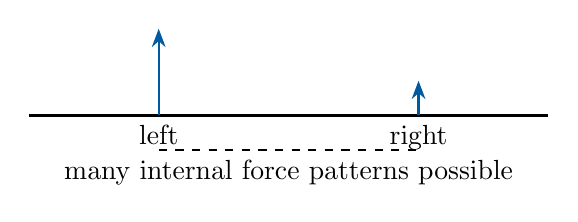
\begin{tikzpicture}[scale=1.1,>=Stealth]
    % Club
    \draw[shaft] (-3,0) -- (3,0);
    % Hands
    \fill[labelpt] (-1.5,0) circle;
    \node[below] at (-1.5,0) {left};
    \fill[labelpt] (1.5,0) circle;
    \node[below] at (1.5,0) {right};
    % Forces: example 1
    \draw[forcevec] (-1.5,0) -- (-1.5,1.0);
    \draw[forcevec] (1.5,0) -- (1.5,0.4);
    % Internal connection
    \draw[dashed] (-1.5,-0.4) -- (1.5,-0.4);
    \node[below] at (0,-0.4) {many internal force patterns possible};
\end{tikzpicture}
\end{center}

The same observed motion of the club could be produced by:
\begin{itemize}
    \item both hands pushing equally,
    \item the lead hand doing most of the work,
    \item the trail hand doing most of the work,
    \item or various combinations of pulling and pushing.
\end{itemize}

The physics does not care which combination was used, as long as the net effect on the club is the same.  
Unfortunately, this means inverse dynamics \emph{cannot} tell you how much each hand really did.

\begin{quote}
\textbf{Inverse dynamics sees only the combined effect of both hands, not the individual contributions.}
\end{quote}

%==========================================================================
\section{Why the Choice of Point Matters}
%==========================================================================

Inverse-dynamics software usually reports the force and torque at a single point on the grip, often the midpoint between the hands.  
This is a convenient place to do the calculation, but it is arbitrary.

If we move the reference point up or down the grip, the reported torque changes.

\subsection*{Diagram 3: Moving the analysis point changes the torque reading}

\begin{center}
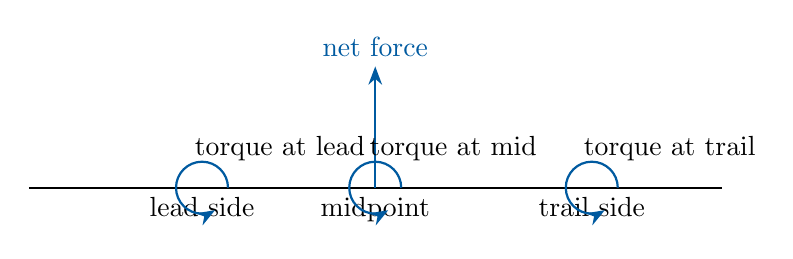
\begin{tikzpicture}[scale=1.1,>=Stealth]
    % Club
    \draw[shaft] (-4,0) -- (4,0);
    % Points
    \fill[labelpt] (-2,0) circle;
    \node[below] at (-2,0) {lead side};
    \fill[refpoint] (0,0) circle;
    \node[below] at (0,0) {midpoint};
    \fill[labelpt] (2.5,0) circle;
    \node[below] at (2.5,0) {trail side};
    % Force (net)
    \draw[forcevec] (0,0) -- (0,1.4) node[above] {net force};
    % Torques
    \draw[couplevec] (-1.7,0) arc (0:300:0.3);
    \node[above] at (-1.1,0.2) {torque at lead};
    \draw[couplevec] (0.3,0) arc (0:300:0.3);
    \node[above] at (0.9,0.2) {torque at mid};
    \draw[couplevec] (2.8,0) arc (0:300:0.3);
    \node[above] at (3.4,0.2) {torque at trail};
\end{tikzpicture}
\end{center}

This is purely geometry: the same net force acting at different locations produces different twisting effects around those locations.

\begin{quote}
\textbf{The sign and size of the reported torque depend on where you choose to look along the grip.}
\end{quote}

So a ``negative torque at the midpoint’’ does not automatically tell you what is happening at either hand.

%==========================================================================
\section{How Force Location Changes the Reported Torque}
%==========================================================================}

Another way to see the problem is to imagine sliding the effective point of force application up and down the grip and watching how the equivalent torque at that point changes.

\subsection*{Diagram 4: Torque value changing as force location slides}

\begin{center}
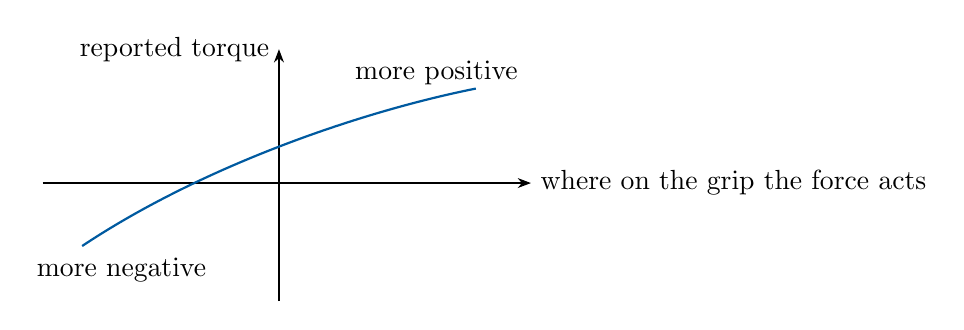
\begin{tikzpicture}[scale=1.0,>=Stealth]
    % Axes
    \draw[axisline,->] (-3,0) -- (3.2,0) node[right] {where on the grip the force acts};
    \draw[axisline,->] (0,-1.5) -- (0,1.7) node[left] {reported torque};
    % Zero-torque line
    \draw[dashed] (-3,0) -- (3,0);
    % Torque trend
    \draw[thick,accent] (-2.5,-0.8) .. controls (-1,0.2) and (1,0.9) .. (2.5,1.2);
    \node at (-2.0,-1.1) {more negative};
    \node at (2.0,1.4) {more positive};
\end{tikzpicture}
\end{center}

Even without changing the motion of the club, the reported torque can:
\begin{itemize}
    \item get larger or smaller,
    \item change sign,
    \item move from what looks like ``twisting against the club’’ to ``twisting with the club’’,
\end{itemize}
depending on where we assume the force acts.

%==========================================================================
\section{Early Backswing and Late Downswing Examples}
%==========================================================================}

\subsection{Early backswing: an upward pull near the trail hand}

Suppose the golfer uses mostly the trail hand to pull the club up early in the backswing, with the force acting closer to that hand than to the midpoint.

\subsection*{Diagram 5: Early-backswing pull near the trail hand}

\begin{center}
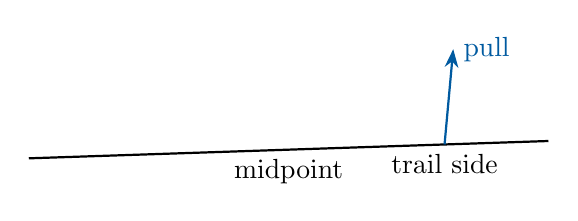
\begin{tikzpicture}[scale=1.1,>=Stealth]
    % Club
    \draw[shaft] (-3,-0.1) -- (3,0.1);
    % Midpoint
    \coordinate (mid) at (0,0);
    \fill[refpoint] (mid) circle;
    \node[below] at (mid) {midpoint};
    % Trail side point
    \coordinate (trail) at (1.8,0.06);
    \fill[labelpt] (trail) circle;
    \node[below] at (trail) {trail side};
    % Upward-ish force
    \draw[forcevec] (trail) -- ($(trail)+(0.1,1.1)$) node[right] {pull};
\end{tikzpicture}
\end{center}

At the midpoint, inverse dynamics might show:
\begin{itemize}
    \item an upward net force, and
    \item a torque with some sign (positive or negative, depending on the sign convention).
\end{itemize}

That torque is telling you that the line of action of the force does not pass through the midpoint—not necessarily that the player is actively twisting.

\subsection{Late downswing: strong rotation, ambiguous torque sign}

In late downswing the club is rotating quickly and has large angular acceleration.  
The overall moment on the club is large.  
Depending on where along the grip the effective force is applied, the torque measured at one point can be positive, while at another plausible point it may be negative—even though the swing motion itself is unchanged.

\subsection*{Diagram 6: Positive here, negative there, same motion}

\begin{center}
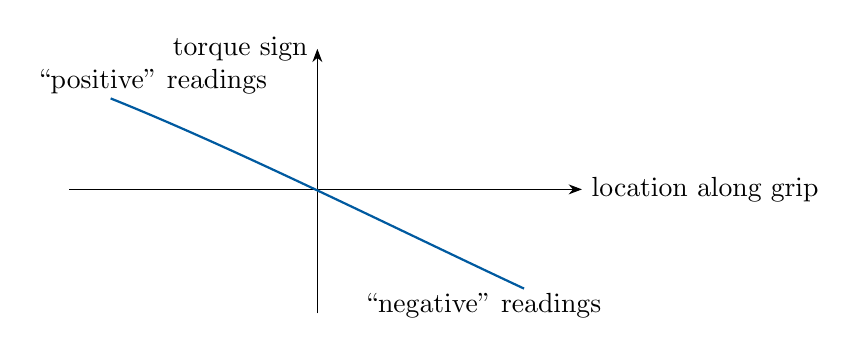
\begin{tikzpicture}[scale=1.05,>=Stealth]
    % Axes
    \draw[axisline,->] (-3,0) -- (3.2,0) node[right] {location along grip};
    \draw[axisline,->] (0,-1.5) -- (0,1.7) node[left] {torque sign};
    % Zero line
    \draw[dashed] (-3,0) -- (3,0);
    % Curve crossing zero
    \draw[thick,accent] (-2.5,1.1) .. controls (-1,0.5) and (1,-0.5) .. (2.5,-1.2);
    % Label regions
    \node at (-2.0,1.3) {``positive'' readings};
    \node at (2.0,-1.4) {``negative'' readings};
\end{tikzpicture}
\end{center}

This is important if you see discussions of ``alpha torque’’ or other named torque quantities.  
The sign of the torque at a chosen point is not a direct look into what the hands are ``trying’’ to do.  
It is partly a matter of where you place the analysis point.

%==========================================================================
\section{What Inverse Dynamics \emph{Can} Tell You}
%==========================================================================}

Used correctly, inverse dynamics is incredibly valuable.  
It can tell you:

\begin{itemize}
    \item How hard the club is being driven overall (in terms of net force and twist).
    \item Where in the swing those loads are highest.
    \item Whether the pattern of loading is smooth or jerky.
    \item How different swings compare in total loading, even if the exact hand contributions remain unknown.
\end{itemize}

It is especially powerful when:
\begin{itemize}
    \item comparing different players or different techniques,
    \item looking at changes before and after a swing change,
    \item or testing equipment differences in a controlled way.
\end{itemize}

%==========================================================================
\section{What Inverse Dynamics \emph{Cannot} Tell You}
%==========================================================================}

There are limits that no amount of clever math can escape, because they are built into the physics of two hands on a club.

Inverse dynamics \textbf{cannot} tell you:
\begin{itemize}
    \item how much the lead hand ``pulled’’ versus the trail hand,
    \item whether one hand pushed while the other resisted,
    \item exactly where on the grip (fingers vs. palms, higher vs. lower) the forces acted,
    \item whether a reported torque is ``good’’ or ``bad’’ in the sense of being a direct twisting action by the player.
\end{itemize}

Those questions require other kinds of data (hand force sensors, EMG, high-resolution grip models) or carefully built assumptions.

\begin{quote}
\textbf{Inverse dynamics is about the club, not about the golfer’s intent.}
\end{quote}

%==========================================================================
\section{How to Use Inverse-Dynamics Results Responsibly}
%==========================================================================}

For coaching and practical analysis, inverse dynamics is best used to:
\begin{itemize}
    \item Understand the overall loading pattern of the club.
    \item Identify phases where the club is being accelerated or decelerated strongly.
    \item Compare how ``aggressively’’ or ``smoothly’’ different swings load the club.
    \item Provide context when combined with other information (video, ground reaction forces, pressure traces, etc.).
\end{itemize}

It is \emph{not} a direct readout of how the hands should feel or what cue to give a player.

Good practice includes:
\begin{itemize}
    \item Treating torque and force time-series as abstract indicators, not literal hand instructions.
    \item Being cautious about using the sign of a torque at a single point to make strong claims about what the hands are doing.
    \item Focusing more on patterns (timing, smoothness, relative peaks) than on isolated samples or single signs.
\end{itemize}

%==========================================================================
\section{Summary for Coaches}
%==========================================================================}

\begin{itemize}
    \item Inverse dynamics starts from the \emph{motion of the club}, not the hands.
    \item It works backwards to find the \emph{overall push and twist} that would create that motion at a chosen point.
    \item Two hands and a grip form a closed system, so many different hand strategies can create the same overall loading.
    \item A torque (twist) shown at the midpoint may appear even if the player never tried to twist; it can arise from where the force acts.
    \item Moving the analysis point along the grip changes the reported torque, sometimes even flipping its sign.
    \item Use inverse dynamics to understand overall load patterns, not to read the golfer’s mind or to assign exact roles to each hand.
\end{itemize}

Inverse dynamics is a powerful lens on the golf swing—but like any lens, it does not show everything.  
Used with a clear understanding of its strengths and limits, it can support better coaching decisions and more realistic conversations about how players actually load the club.

\end{document}
